% ── Section 1: Introduction ───────────────────────────────
\section{Introduction}
\label{sec:introduction}

Coastal ocean monitoring stations produce long and biologically informative time series, but they
are rarely complete: sensor outages, maintenance windows, and storm damage interrupt
the record, often precisely when the underlying signal is most dynamic and most scientifically
interesting. Reconstructing these historical gaps matters both for day-to-day monitoring and for
any downstream scientific interpretation of the record. What operational networks need is not a
one-off fix for a single station or variable, but a workflow that can be reapplied each time a
new sensor or a new gap appears \citep{moritz2017imputets}.

This report develops such a workflow for the Centro de Estudios Avanzados en Zonas \'{A}ridas
(CEAZA) network \citep{ceazamet_network} at Tongoy Bay, Chile
($\sim$30.3\textdegree{}S, 71.6\textdegree{}W; Figure~\ref{fig:site-context}), a Humboldt Current
upwelling site \citep{montecino2009humboldt} that hosts a scallop (\textit{Argopecten
purpuratus}) aquaculture industry whose production is closely tied to local phytoplankton
dynamics and to upwelling-driven variability in oxygen, temperature, and pH
\citep{ramajo2019scallops}. Two sensors on the Tongoy buoy (BTG) anchor the study: an in-situ
chlorophyll-\textit{a} (\chl{}) fluorometer, the primary case study, and a dissolved-oxygen
sensor, a second case study that tests how well the workflow transfers to a physically distinct
variable. Both records span 2015--2026 and share the buoy's missingness structure, including a
common 256-day station-wide outage during the 2020 pandemic; chlorophyll's daily record is 24.5\% missing and oxygen's is
27.8\% missing (Section~\ref{sec:data}).

Reconstructing a nearshore biological signal like \chl{} is harder than a generic gap-filling
problem, and the report treats the reasons as questions to answer:
\begin{itemize}
    \item \textbf{How strong are the simple baselines?} Linear interpolation and climatology are the floor every method must clear.
    
    \item \textbf{Do external satellite and physical products help?} Regional ocean-colour and reanalysis fields (wind, current, sea surface temperature) are continuously available during a gap, but their resolution may be too coarse for a nearshore signal.

    \item \textbf{Can a zero-shot foundation model provide an alternative?} Such models require no station-specific training and no feature engineering, which is attractive operationally.

    \item \textbf{Where do the methods fail?} The regimes of greatest interest --- short chlorophyll blooms and the tails of the oxygen distribution --- are where imputation is hardest.
\end{itemize}
 
One principle organises all of the evidence. Methods are ranked only on artificial gaps: observed values are hidden, each method reconstructs them, and the reconstruction is
scored against the withheld truth. The stations' real gaps have no ground truth, so any
reconstruction of them can be inspected for plausibility and is useful for the research center activities, but never used to rank methods. \\
The report makes two contributions.

First, it benchmarks five comparator groups for daily in-situ Chl a under an artificial-gap protocol: simple temporal baselines, a target-only Gaussian-process
smoother, an engineered tabular model using only external predictors, a gap-edge residual model
conditioned on the observations bounding each gap, and a pretrained time-series foundation model
(TS-ICL) applied zero-shot, reporting which method wins, where, and why.
Second, it carries the same target-definition, gap-audit, and model-ladder workflow through to a
second sensor, dissolved oxygen (Section~\ref{sec:oxygen}), so that the benchmark itself, and not
just the chlorophyll result, is the reusable product CEAZA can reapply to further sensors and
stations.

Section~\ref{sec:data} describes both case studies' data and target construction;
Section~\ref{sec:methodology} defines the shared benchmark;
Section~\ref{sec:chl_results} presents the chlorophyll results in full;
Section~\ref{sec:oxygen} presents the more compact oxygen case;
Section~\ref{sec:synthesis} compares what transfers between the two; and
Section~\ref{sec:limitations_future} closes with limitations and research directions.
Appendix~\ref{sec:appendix_repro} gives the compact reproducibility details and backing tables,
while the accompanying code repository contains the complete implementation and raw outputs.

\begin{figure}[h]
  \centering
  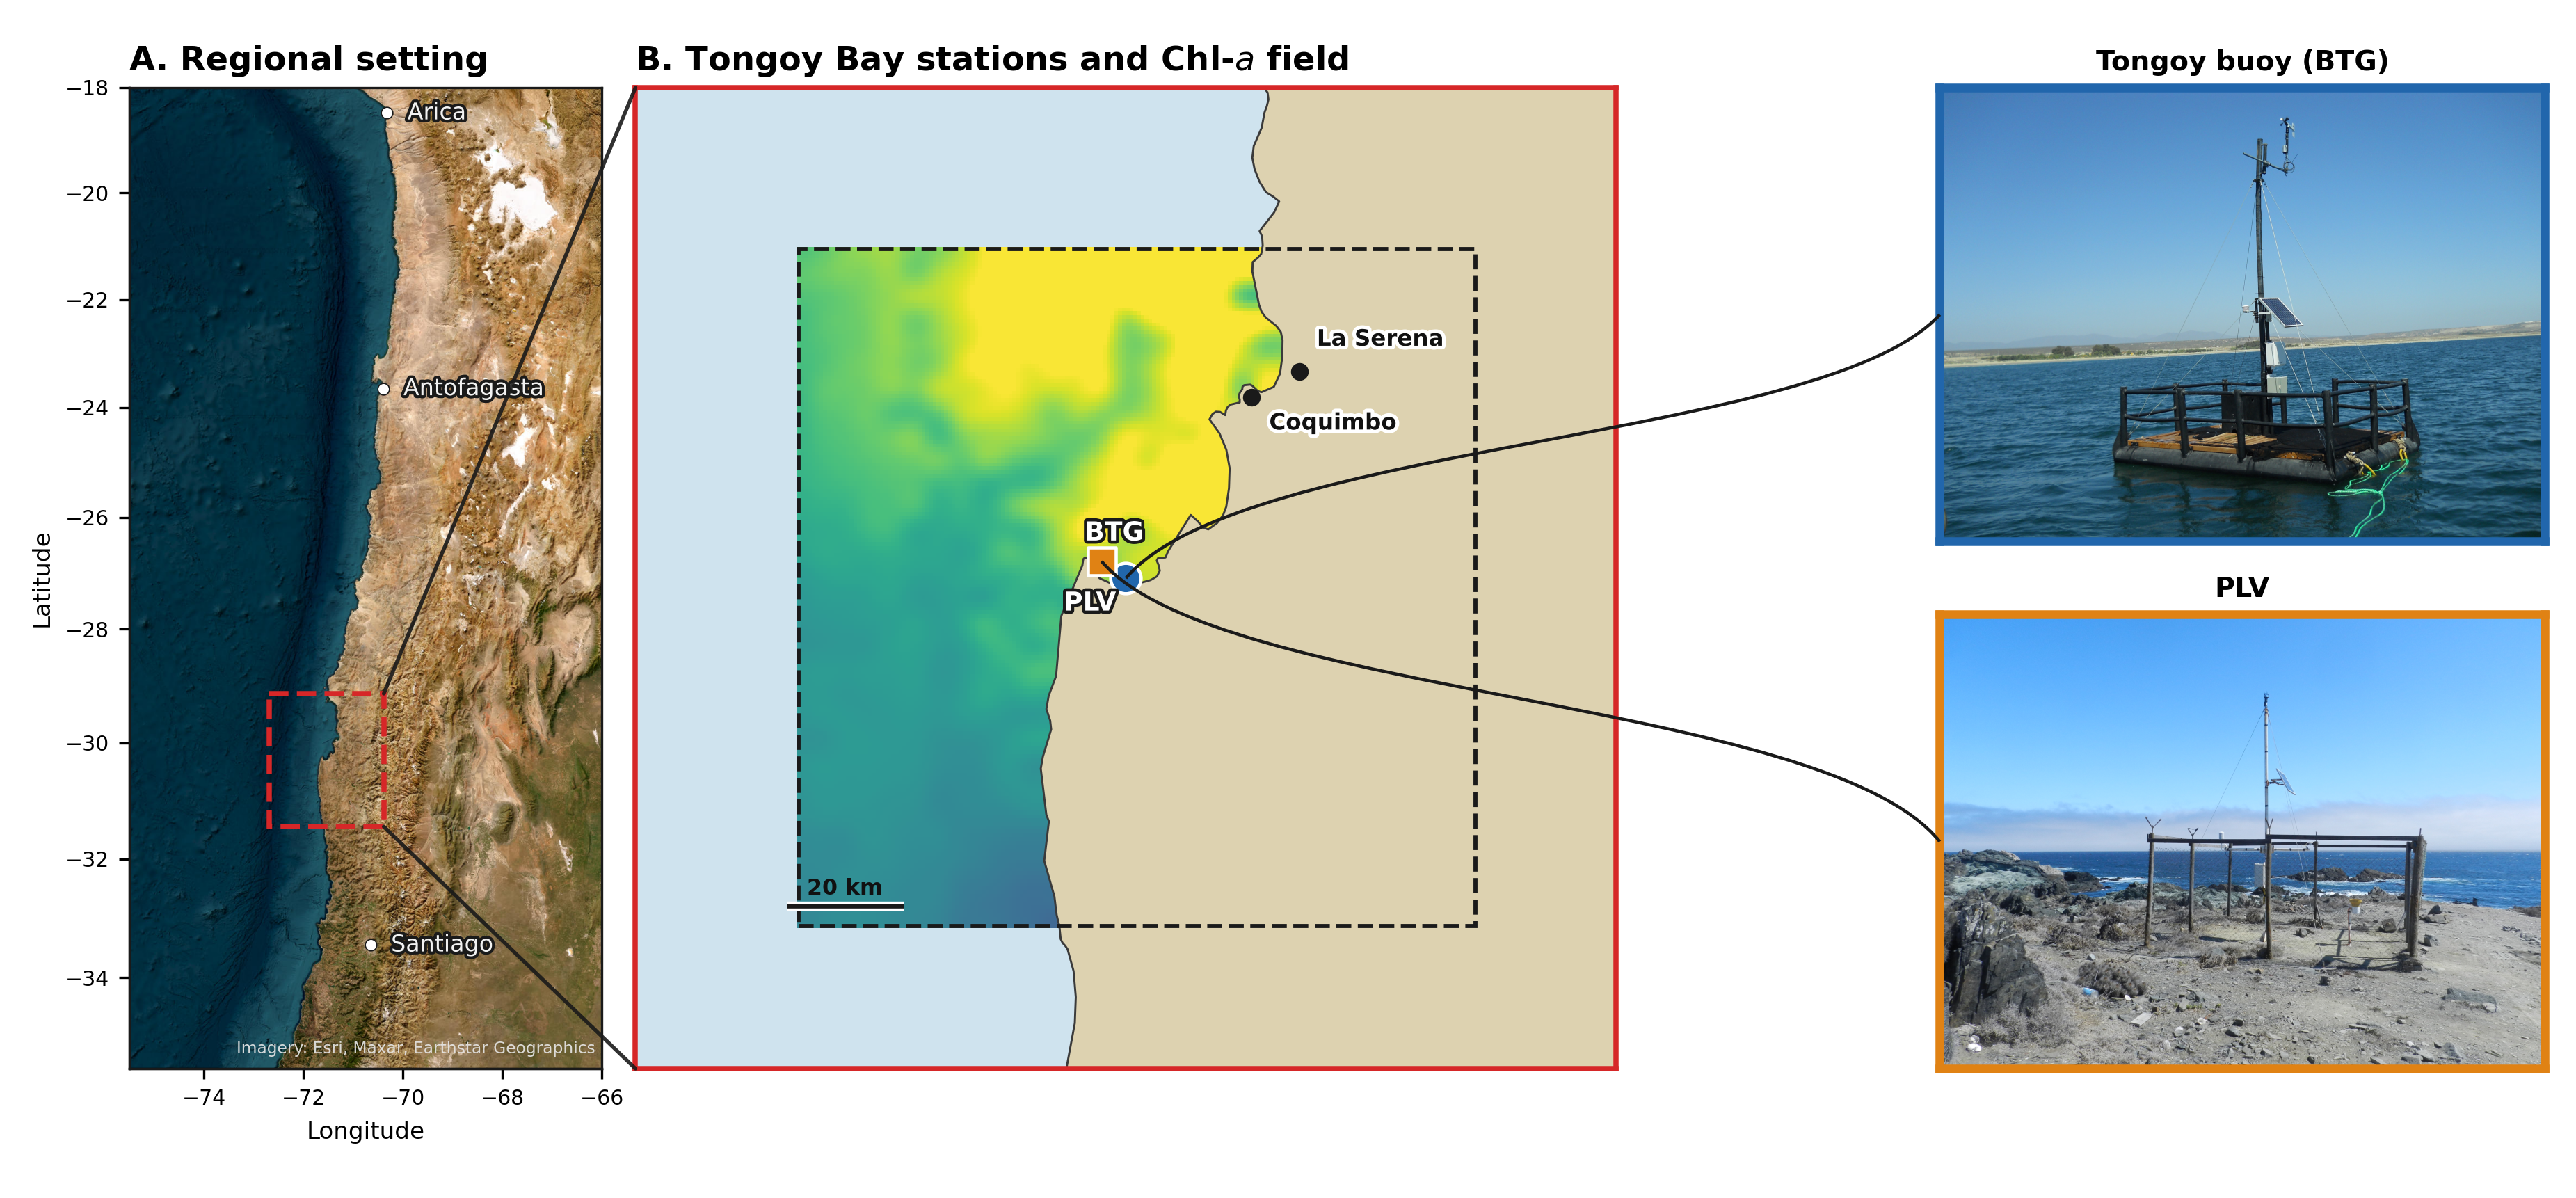
\includegraphics[width=\textwidth]{figures/fig1_site_context.png}
  \caption{Study site and monitoring context. (A) Regional setting on the north-central
  Chilean coast; (B) Tongoy Bay:
  the Tongoy buoy (BTG, carrying the chlorophyll and dissolved-oxygen sensors), the PLV
  meteorological station, the satellite/reanalysis extraction domain (dashed box), and a
  representative satellite Chl-\textit{a} field (2021-01-17), with field photographs of both installations.}
  \label{fig:site-context}
\end{figure}